\documentclass[12pt,a4paper]{article}
\usepackage{composites2019}

\begin{document}
\thispagestyle{empty}

\vspace*{-3.4cm}
\begin{table}[!h]
\begin{tabular}{r}
\hspace*{5.5cm} \scriptsize \textsf{7th ECCOMAS Thematic Conference on the Mechanical Response of Composites} \\
\hspace*{5.5cm} \scriptsize \textsf{ COMPOSITES 2019} \\
\hspace*{5.5cm} \tiny \textsf{A. Turon, P. Maimí \& M. Fagerström (Editors)}
\end{tabular}
\end{table}

\begin{center}
\title{ESTIMATING THE AVERAGE SIZE OF FIBER/MATRIX INTERFACE CRACKS IN UD AND CROSS-PLY LAMINATES}
\end{center}
\begin{center}
\textbf{\underline{Luca Di Stasio}$^{1,2,*}$, Janis Varna$^{1}$, Zoubir Ayadi$^{2}$} \\ [7pt]
\small{$^1$~Lule\aa\ University of Technology, University Campus, SE-97187 Lule\aa, Sweden}  \\  [2pt]  
\small{$^2$~Universit\'e de Lorraine, EEIGM, IJL, 6 Rue Bastien Lepage, F-54010 Nancy, France}  \\  [2pt]
\small{$^*$~\texttt{luca.di.stasio@ltu.se}} \\
\end{center}


\paragraph{Keywords:} Modeling, Experimental validation, Industrial applications.

\paragraph{Summary:} \textit{This document provides information and instructions for preparing the (optional) full-length paper for the COMPOSITES 2019 Conference (September 18-20, 2019 in Girona, Spain).}

\section{INTRODUCTION}

The Conference publication will consist of a pen drive containing papers of the contributions received and a printed Book of Abstracts containing a one page version of the accepted abstracts. The authors must submit a full-length paper (max. 12 pages) using the same format of this template. Submission of a full-length paper is not mandatory but authors are strongly encouraged to send it before June 27, 2019.

The deadline date for early registration date is April 30, 2019. Presenting authors must register by June 13, 2019. Papers with authors not registered by this date will be removed from the final program.
Registration closes on September 5, 2019. Further information can be found at the conference website: \texttt{www.composites2019.udg.edu}

\section{GENERAL SPECIFICATIONS}
The full-length paper must be written in English and should have a maximum length of 12 pages.

\section{TITLE, AUTHORS, KEY WORDS}
The first page must contain the Title, Author(s), Affiliation(s), Key words and the Summary. The Introduction must begin immediately below, following the format of this template.

\subsection{Title}
The title should be written with all capital letters.
\subsection{Author}
The author's name should include first name, middle initial and surname.
\subsection{key words}
Please, write no more than three keywords.

\section{FIGURES}

All figures are automatically numbered consecutively and captioned, and should be embedded in the Paper, see for example Figure~\ref{fig:Claustre}.

\begin{figure}[!h]
 \centering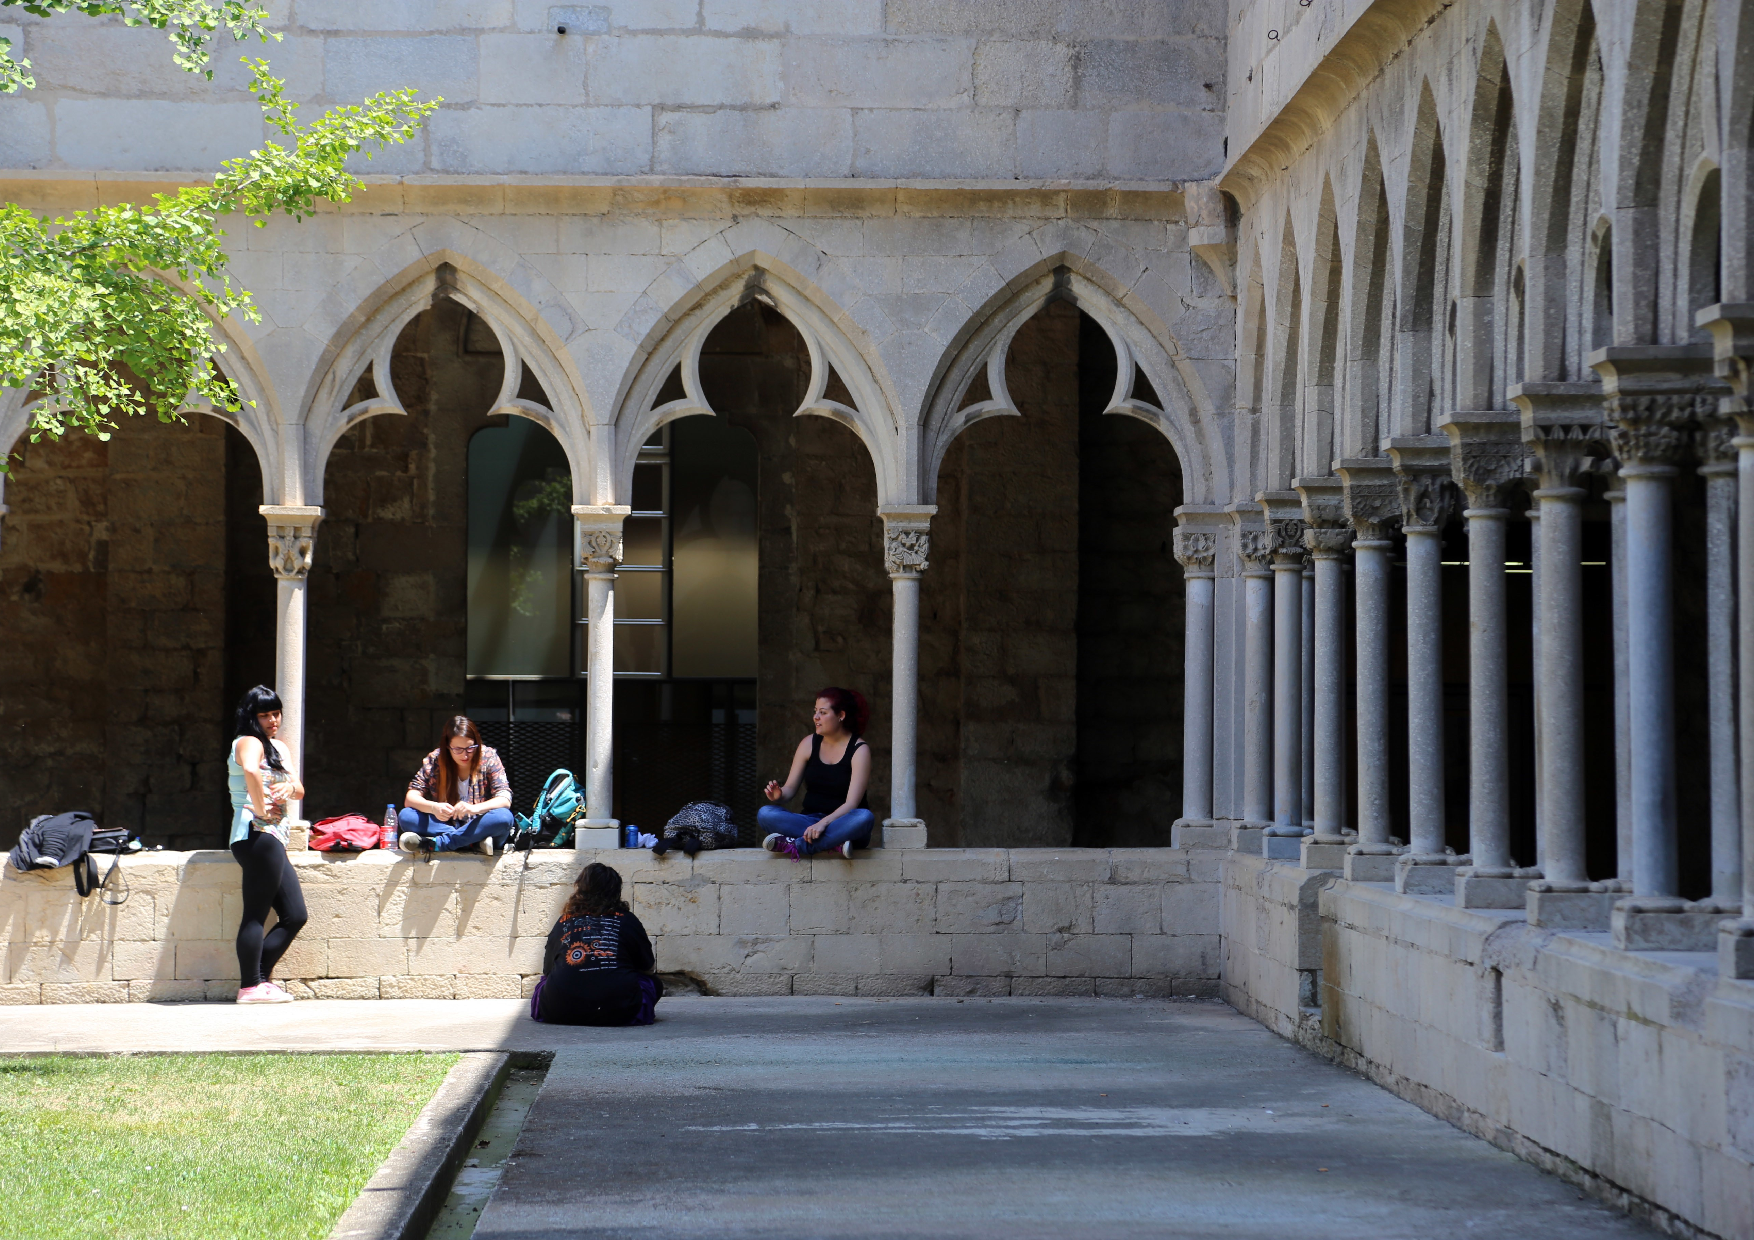
\includegraphics[width=0.65\linewidth]{Claustre.pdf}
 \caption{The cloister of the convent of St. Domènec, which is the venue of this conference.}
 \label{fig:Claustre}
\end{figure}

\section{EQUATIONS}

A displayed equation is automatically numbered, using Arabic numbers in parentheses.
The following example is a single line equation:

\begin{align}
 Ax = b
\end{align}

The next example is a multi-line equation:
\begin{equation}
 \begin{aligned}
  Ax &=b \\
  Ax &=b
 \end{aligned}
\end{equation}


\section{TABLES}
All tables are automatically numbered consecutively and captioned.

\begin{table}[!h]
\centering
\caption{Example of the construction of a table.}
\setlength{\arrayrulewidth}{2\arrayrulewidth}
\begin{tabular}{ccc}
\hline
C11 & C12 & C13 \\
C21 & C22 & C23 \\
C31 & C32 & C33 \\
C41 & C42 & C43 \\
C51 & C52 & C53 \\
\hline
\end{tabular}
\end{table}


\section{FORMAT OF REFERENCES}
References should be quoted in the text by numbers \cite{Barbero,Pimenta} and grouped together at the end of the Abstract in numerical order as shown in these instructions. Use the $unsrt$ style either with the $BibTeX$ or the $\backslash$$bibitem$ format.

\section{CONCLUSIONS}

We are looking forward to receiving your contributions for this conference.

\bibliographystyle{unsrt}
\begin{thebibliography}{10}

\bibitem{Barbero} E.J. Barbero, \textit{Finite Element Analysis of Composite Materials}. CRC Press, Boca Raton, 2008.
\bibitem{Pimenta} S. Pimenta, S.T. Pinho, The effect of recycling on the mechanical response of carbon fibres and their composites. \textit{Composite Structures}, \textbf{94}, 3669-3684, 2012.

\end{thebibliography}

\end{document}

